\section{最適制御と確率的推定}

小さな台車を目標位置で静止させる制御を考える。位置偏差をすばやく 0 に近づけたいが、モータ電流や推力を大きくしすぎると発熱、飽和、消費電力の問題が生じる。また、位置センサには分解能とノイズがあり、速度を直接測れない場合には、測定値を単純に差分するとノイズが入力へ入りやすい。したがって設計者が同時に扱うべき量は、目標からのずれ、アクチュエータの使用量、測定の信頼度、モデル予測の信頼度である。

本節では、この二つの妥協を線形モデルの上で定式化する。まず、状態が利用でき、入力に明示的な飽和や上下限制約がない場合に、状態偏差と入力偏差の重み付き和を最小にする LQR を導く。次に、状態の一部しか測れず、測定値とモデルに不確かさがある場合に、予測と測定を共分散で重み付けして状態を推定する Kalman フィルタを導く。いずれも、平衡点または目標軌道の近傍で線形化したモデルを用いる基準設計であり、重み行列や共分散行列は、メートル、メートル毎秒、ニュートン、ボルトなどの異なる物理単位を共通の評価量へ換算する役割を持つ。

\subsection{線形最適制御}

状態フィードバックでは、極をどこに置くかを設計者が選んだ。しかし、台車を「速く止める」だけなら極を左へ動かせばよいとしても、同時に「入力をどれだけ節約するか」は極の位置だけでは直接指定しにくい。ここでは状態偏差を $x(t)\in\R^n$、入力偏差を $u(t)\in\R^m$ とし、たとえば $x$ の成分には位置偏差や速度偏差、$u$ にはモータ電流や推力の偏差が入ると考える。対象は動作点まわりで線形化され、行列 $A$ と $B$ は時不変、初期状態は既知、入力飽和はこの段階では扱わないと仮定する。この条件で、線形系
\begin{equation}
  \dot{x}=Ax+Bu
\end{equation}
に対する評価関数
\begin{equation}
  J=\int_0^\infty \{x(t)^\T Qx(t)+u(t)^\T Ru(t)\}\,\dd t
\end{equation}
を置く。$Q=Q^\T\ge0$ は状態のずれへの重み、$R=R^\T>0$ は入力への重みである。積分の中の $x^\T Qx$ と $u^\T Ru$ は同じ評価率の単位を持つように選ぶ。したがって、位置をメートル、速度をメートル毎秒、入力をニュートンで表すなら、$Q$ と $R$ の各成分はそれぞれの二乗単位を評価率へ換算する係数である。$Q$ を大きくすればずれを強く嫌い、$R$ を大きくすれば入力を節約する。

入力を $u=-Kx$ と置くと、閉ループは $\dot{x}=(A-BK)x$ になる。LQR は、すべての安定化ゲインの中から $J$ を最小にする $K$ を選ぶ。最適ゲインは
\begin{equation}
  K=R^{-1}B^\T P
\end{equation}
であり、$P$ は代数リカッチ方程式
\begin{equation}
  A^\T P+PA-PBR^{-1}B^\T P+Q=0
  \label{eq:care}
\end{equation}
を満たす半正定値の安定化解である。$Q>0$ のように状態全体が十分に罰せられる場合には $P>0$ になる。最適コストは
\begin{equation}
  V(x)=x^\T P x
\end{equation}
となる。前節のリアプノフ関数が安定性を評価する関数だったのに対し、ここでの $V$ は「これから必要になる最小コスト」を表す関数でもある。

有限時間を対象にする場合は、終端時刻 $T$ までの評価
\begin{equation}
  J=x(T)^\T S x(T)+\int_0^T(x^\T Qx+u^\T Ru)\,\dd t
\end{equation}
を最小にする。ここで $S\ge0$ は終端時刻で残った状態偏差をどの程度重く評価するかを表す終端重みである。リカッチ方程式は終端条件 $P(T)=S$ から時間を逆向きに解く微分方程式になる。この有限ホライズンの考え方は後で MPC へ進むための前提だが、ここではまだ制約のない連続時間最適制御として理解しておく。

\subsection{変分法と最適性条件}

最適制御では、時刻ごとの入力値を一つずつ選ぶのではなく、区間全体の入力関数 $u(\cdot)$ を選ぶ。したがって評価関数は、数 $u$ の関数ではなく、関数 $u(\cdot)$ を受け取って数を返す汎関数である。典型的な有限時間問題は
\begin{align}
  J[u]
  &=
  \phi(x(T))
  +\int_0^T \ell(x(t),u(t),t)\,\dd t,\\
  \dot{x}(t)&=f(x(t),u(t),t),
  \qquad x(0)=x_0
  \label{eq:oc-general-problem}
\end{align}
で表される。$\ell$ は途中で支払うランニングコスト、$\phi$ は終端コストである。状態 $x(t)\in\R^n$ と入力 $u(t)\in\R^m$ は時刻に依存する関数であり、制御入力を少し変えると、状態軌道全体も変わる。この「関数を少し変えたときの評価関数の一次の変化」を調べる操作を変分という。

許される小さな入力変化を $\eta(t)$ とし、
\begin{equation}
  u_\varepsilon(t)=u(t)+\varepsilon \eta(t)
\end{equation}
と置く。対応する状態を $x_\varepsilon(t)$ と書くと、第一変分は
\begin{equation}
  \delta J
  =
  \left.\frac{\dd}{\dd\varepsilon}J[u_\varepsilon]\right|_{\varepsilon=0}
  \label{eq:first-variation}
\end{equation}
で定義される。通常の一変数関数で最小値の候補が $F'(z)=0$ を満たすように、制約のない十分滑らかな最適入力では、すべての許される $\eta$ に対して $\delta J=0$ が必要条件になる。この条件は必要条件であって、凸性や正定性がなければ大域最小性までは保証しない。

変分の基本形は、入力制御を含まない曲線最適化で確認できる。軌道 $x(t)$ そのものを選び、
\begin{equation}
  J[x]=\int_0^T L(x(t),\dot{x}(t),t)\,\dd t
\end{equation}
を最小にする問題を考える。端点 $x(0)$、$x(T)$ を固定し、$x_\varepsilon=x+\varepsilon \xi$、$\xi(0)=\xi(T)=0$ と置くと
\begin{align}
  \delta J
  &=
  \int_0^T
  \left(
    \frac{\partial L}{\partial x}\xi
    +\frac{\partial L}{\partial \dot{x}}\dot{\xi}
  \right)\,\dd t\\
  &=
  \int_0^T
  \left(
    \frac{\partial L}{\partial x}
    -\frac{\dd}{\dd t}\frac{\partial L}{\partial \dot{x}}
  \right)\xi\,\dd t
  +
  \left[
    \frac{\partial L}{\partial \dot{x}}\xi
  \right]_0^T.
\end{align}
端点固定により境界項は 0 である。任意の $\xi$ に対して $\delta J=0$ となるには、括弧内が各時刻で 0 でなければならない。よって Euler--Lagrange 方程式
\begin{equation}
  \frac{\partial L}{\partial x}
  -\frac{\dd}{\dd t}
  \frac{\partial L}{\partial \dot{x}}
  =0
  \label{eq:euler-lagrange-entry}
\end{equation}
を得る。これは「最適な曲線では、許される微小な曲線変化に対して評価関数の一次変化が消える」という条件である。力学で Euler--Lagrange 方程式が現れるのも同じ変分の構造による。

制御問題では、軌道 $x$ は自由に選べず、状態方程式 $\dot{x}=f(x,u,t)$ に従う。この動的制約を扱うため、随伴変数 $\lambda(t)\in\R^n$ を導入し、拡張された汎関数
\begin{equation}
  \bar{J}
  =
  \phi(x(T))
  +\int_0^T
  \left\{
    \ell(x,u,t)
    +\lambda^\T\bigl(f(x,u,t)-\dot{x}\bigr)
  \right\}\,\dd t
\end{equation}
を考える。最適軌道では $f-\dot{x}=0$ なので、$\bar{J}$ と $J$ の値は一致する。$x$ と $u$ の変分を取り、$\lambda^\T\dot{x}$ の項を部分積分して一次の項を集めると、Pontryagin の Hamiltonian
\begin{equation}
  \mathcal{H}(x,u,\lambda,t)
  =
  \ell(x,u,t)+\lambda^\T f(x,u,t)
  \label{eq:pontryagin-hamiltonian}
\end{equation}
により、内部点の必要条件は
\begin{align}
  \dot{x}&=\frac{\partial \mathcal{H}}{\partial \lambda}
  =f(x,u,t),
  \label{eq:pmp-state}\\
  -\dot{\lambda}&=\frac{\partial \mathcal{H}}{\partial x},
  \label{eq:pmp-costate}\\
  0&=\frac{\partial \mathcal{H}}{\partial u},
  \label{eq:pmp-stationarity}\\
  \lambda(T)&=\frac{\partial \phi}{\partial x}(x(T)).
  \label{eq:pmp-terminal}
\end{align}
となる。$\lambda$ は状態を少し変えたときに将来の最小コストがどれだけ変わるかを表す感度であり、随伴変数または共状態と呼ばれる。状態方程式は初期条件 $x(0)=x_0$ から前向きに進み、随伴方程式は終端条件 \weq{pmp-terminal} から後ろ向きに決まる。したがって、最適制御問題は一般に二点境界値問題になる。入力制約がない滑らかな場合は \weq{pmp-stationarity} を使うが、入力に上下限や不等式制約がある場合は、Hamiltonian を許容集合上で最小にする条件や KKT 条件へ置き換わる。

同じ問題の別表現が動的計画法である。時刻 $t$、状態 $x$ から終端までに達成できる最小残りコストを値関数
\begin{equation}
  V(t,x)=
  \min_{u(\cdot)}
  \left\{
    \phi(x(T))
    +\int_t^T \ell(x(\tau),u(\tau),\tau)\,\dd \tau
  \right\}
  \label{eq:value-function-entry}
\end{equation}
と定義する。短い時間幅 $h>0$ だけ先へ進めると、最適性の原理より
\begin{equation}
  V(t,x)=
  \min_{u(\cdot)}
  \left\{
    \int_t^{t+h}\ell(x(\tau),u(\tau),\tau)\,\dd \tau
    +V(t+h,x(t+h))
  \right\}
  \label{eq:dynamic-programming-principle}
\end{equation}
が成り立つ。右辺は、最初の短い区間で支払うコストと、その後の最小残りコストの和である。$h$ を十分小さくし、$x(t+h)=x+h f(x,u,t)+o(h)$ を代入して Taylor 展開すると
\begin{align}
  0=
  \min_u
  \left\{
    \ell(x,u,t)
    +\frac{\partial V}{\partial t}(t,x)
    +\frac{\partial V}{\partial x}(t,x)^\T f(x,u,t)
  \right\}
  \label{eq:hjb-entry}
\end{align}
を得る。これが Hamilton--Jacobi--Bellman 方程式であり、終端条件は $V(T,x)=\phi(x)$ である。Pontryagin の条件が一つの最適軌道に沿った必要条件を与えるのに対し、HJB 方程式は全状態に対する値関数を求める方程式である。滑らかな値関数が得られる場合、両者は
\begin{equation}
  \lambda(t)=
  \frac{\partial V}{\partial x}(t,x(t))
  \label{eq:costate-value-gradient}
\end{equation}
で結びつく。

LQR では、この一般形が閉じた行列方程式に落ちる。線形系 $f=Ax+Bu$、二次コスト
\begin{equation}
  \ell=x^\T Qx+u^\T Ru,
  \qquad
  \phi=x^\T Sx
\end{equation}
を用いると、Hamiltonian は
\begin{equation}
  \mathcal{H}
  =
  x^\T Qx+u^\T Ru+\lambda^\T(Ax+Bu)
\end{equation}
であり、停留条件から
\begin{equation}
  0=2Ru+B^\T\lambda,
  \qquad
  u=-\frac{1}{2}R^{-1}B^\T\lambda
\end{equation}
を得る。一方、HJB で値関数を $V(t,x)=x^\T P(t)x$ と置けば
\begin{equation}
  \lambda=\partial_x V=2P(t)x
\end{equation}
なので、最適入力は
\begin{equation}
  u=-R^{-1}B^\T P(t)x
\end{equation}
となる。さらに HJB 方程式の二次形式の係数を 0 と置くことでリカッチ微分方程式が得られ、無限ホライズンではその定常解が代数リカッチ方程式になる。したがって、変分、Pontryagin の条件、動的計画法、HJB は別々の公式ではなく、LQR のリカッチ方程式へ至る同じ最適性の構造を異なる表現で見ている。

最後に、一次元の積分器でこの接続を確認する。対象を
\begin{equation}
  \dot{x}=u,
  \qquad x(0)=x_0
\end{equation}
とし、評価関数を
\begin{equation}
  J=sx(T)^2+\int_0^T r u(t)^2\,\dd t,
  \qquad s\ge0,\quad r>0
  \label{eq:scalar-integrator-cost}
\end{equation}
とする。Hamiltonian は
\begin{equation}
  \mathcal{H}=r u^2+\lambda u
\end{equation}
である。最適性条件は
\begin{align}
  \dot{x}&=u,\\
  -\dot{\lambda}&=0,\\
  0&=2ru+\lambda,\\
  \lambda(T)&=2s x(T)
\end{align}
である。したがって $\lambda$ は定数で、$u=-\lambda/(2r)$ も定数になる。終端条件に $x(T)=x_0+Tu$ を代入すると
\begin{align}
  \lambda
  &=2s\left(x_0-\frac{T}{2r}\lambda\right),\\
  \lambda\left(1+\frac{sT}{r}\right)&=2s x_0,\\
  u^*&=-\frac{s}{r+sT}x_0
\end{align}
を得る。同じ結果を HJB から導く。$V(t,x)=P(t)x^2$ と置いたとき
\begin{equation}
  0=\min_u\{r u^2+\dot{P}x^2+2P xu\}
\end{equation}
であり、$u^*=-(P/r)x$、さらに
\begin{equation}
  \dot{P}=\frac{P^2}{r},
  \qquad
  P(T)=s
\end{equation}
となる。このスカラーのリカッチ方程式を解くと
\begin{equation}
  P(t)=\frac{sr}{r+s(T-t)}
  \label{eq:scalar-riccati-solution}
\end{equation}
である。したがって $t=0$ では
\begin{equation}
  u^*(0)=-\frac{P(0)}{r}x_0
  =-\frac{s}{r+sT}x_0
\end{equation}
となり、Pontryagin の条件から得た入力と一致する。この小さな例では、随伴変数、値関数の勾配、リカッチ方程式が同じ最適性条件の別表現であることが直接確認できる。

\subsection{確率とノイズ}

ここまでの制御では、状態 $x$ が分かっているか、少なくともオブザーバで滑らかに推定できると考えた。台車の例では、位置センサから位置は読めても、速度は測れないことが多い。さらに、センサの分解能や電気的な揺らぎにより、測定値をそのまま真値とみなすと入力が細かく振れる。測定値 $y$ を
\begin{equation}
  y=Cx+v
\end{equation}
と書くと、$v$ は測定ノイズである。$y$ の単位は測定量の単位であり、位置センサならメートル、角度センサならラジアンである。平均が 0、分散が $\sigma^2$ のノイズなら
\begin{equation}
  E[v]=0,
  \qquad
  E[v^2]=\sigma^2
\end{equation}
である。多次元では共分散行列
\begin{equation}
  R=E[vv^\T]
\end{equation}
がノイズの大きさと相関を表す。$R$ の $(i,j)$ 成分は、測定 $y_i$ と $y_j$ の単位の積を持つ。

モデルにも不確かさがある。摩擦、坂道、外乱、離散化誤差をすべて正確には書けないため、離散時間モデルを
\begin{align}
  x_{k+1}&=A x_k+B u_k+w_k,\\
  y_k&=C x_k+v_k
\end{align}
と書き、$w_k$ の共分散を $Q$、$v_k$ の共分散を $R$ とする。この導入では記号を簡潔に $Q,R$ と書くが、後の詳細な導出では LQR の重みと区別するためにプロセスノイズ共分散を $Q_w$、測定ノイズ共分散を $R_v$ と書く。$Q$ の成分は状態成分の単位の積、$R$ の成分は測定成分の単位の積を持つ。$Q$ が大きいほどモデルを疑い、$R$ が大きいほどセンサを疑う。推定とは、この二つの信頼度を使って状態を更新することである。

\subsection{カルマンフィルタ}

まず1次元で、予測値と測定値の混ぜ方を確認する。事前推定値を $\hat{x}^-$、その分散を $P^-$、測定値を $y$、測定ノイズ分散を $R$ とする。$x$ が位置なら $P^-$ と $R$ は平方メートルの単位を持ち、値が大きいほどその情報を信じにくいことを表す。更新後の推定値を
\begin{equation}
  \hat{x}=\hat{x}^-+K(y-\hat{x}^-)
\end{equation}
と置くと、$K$ は測定をどれだけ信じるかを表す。誤差分散を最小にするゲインは
\begin{equation}
  K=\frac{P^-}{P^-+R}
\end{equation}
である。事前分散が大きいほど測定を信じ、測定ノイズが大きいほど事前値を信じる。

多次元のカルマンフィルタは、線形モデルに対する予測と更新で書ける。
\begin{align}
  \hat{x}_{k|k-1}&=A\hat{x}_{k-1|k-1}+Bu_{k-1},\\
  P_{k|k-1}&=AP_{k-1|k-1}A^\T+Q,\\
  K_k&=P_{k|k-1}C^\T(CP_{k|k-1}C^\T+R)^{-1},\\
  \hat{x}_{k|k}&=\hat{x}_{k|k-1}+K_k(y_k-C\hat{x}_{k|k-1}),\\
  P_{k|k}&=(I-K_kC)P_{k|k-1}.
\end{align}
ここで $P$ は推定誤差の共分散である。カルマンフィルタは、線形ガウス系では平均二乗誤差を最小にする推定器である。

LQR は状態が利用可能である場合の最適状態フィードバックであり、Kalman フィルタは線形確率モデルにおける状態推定器である。線形ガウス仮定のもとでは、Kalman フィルタで得た $\hat{x}$ を LQR の状態フィードバックへ入力する構成が LQG 制御を与える。本節では、対象および推定器を線形として扱う。

\subsection{LQR を平方完成で導く}

極配置では、閉ループ極を指定して応答の速さや減衰を設計した。しかし、台車の位置をすばやく戻したい一方で加える力には上限がある、あるいはモータの角度誤差を小さくしたい一方で電流を大きくしすぎたくない、という設計では、極だけでは「状態のずれ」と「入力の大きさ」をどの割合で許すかを数値で比較できない。極を速く置けば偏差は早く消えるが、一般に入力は大きくなり、飽和や発熱の制約に近づく。そこで、状態偏差を二次形式 $x^\T Qx$、入力努力を $u^\T Ru$ として同じ評価関数へ入れ、重み $Q,R$ によってその交換条件を明示する。平方完成は、この二次評価の中で入力 $u$ がどの値を選ぶと残りコストを最も小さくするかを直接取り出すために用いる。

\begin{theorem}[連続時間 LQR のリカッチ方程式]
$(A,B)$ が可安定で、$(A,Q^{1/2})$ が可検出である線形系 $\dot{x}=Ax+Bu$ に対し、評価関数
\begin{equation}
  J=\int_0^\infty (x^\T Qx+u^\T Ru)\,\dd t,
  \qquad Q=Q^\T\ge0,
  \quad R=R^\T>0
\end{equation}
を最小にする状態フィードバックは
\begin{equation}
  u=-R^{-1}B^\T Px
\end{equation}
であり、$P$ は代数リカッチ方程式
\begin{equation}
  A^\T P+PA-PBR^{-1}B^\T P+Q=0
\end{equation}
を満たす半正定値の安定化解である。
\end{theorem}

\begin{derivation}
最適な残りコストが二次形式
\begin{equation}
  V(x)=x^\T Px
\end{equation}
で表せると仮定する。最適制御の動的計画法、すなわち Hamilton--Jacobi--Bellman 方程式より
\begin{equation}
  0=\min_u\{x^\T Qx+u^\T Ru+\dot{V}(x)\}
\end{equation}
である。$\dot{x}=Ax+Bu$ なので
\begin{align}
  \dot{V}
  &=\dot{x}^\T Px+x^\T P\dot{x}\\
  &=(Ax+Bu)^\T Px+x^\T P(Ax+Bu)\\
  &=x^\T A^\T Px+u^\T B^\T Px+x^\T PAx+x^\T PBu.
\end{align}
スカラーは転置しても同じなので $u^\T B^\T Px=x^\T PBu$ である。したがって
\begin{equation}
  \dot{V}=x^\T(A^\T P+PA)x+2u^\T B^\T Px.
\end{equation}
HJB 方程式の中身は
\begin{equation}
  x^\T Qx+x^\T(A^\T P+PA)x+u^\T Ru+2u^\T B^\T Px
\end{equation}
である。$u$ に関する部分を平方完成する。
\begin{align}
  u^\T Ru+2u^\T B^\T Px
  &=(u+R^{-1}B^\T Px)^\T R(u+R^{-1}B^\T Px)\\
  &\quad -x^\T PBR^{-1}B^\T Px.
\end{align}
第一項は $R>0$ より非負であり、最小にするには
\begin{equation}
  u+R^{-1}B^\T Px=0
\end{equation}
とすればよい。よって
\begin{equation}
  u=-R^{-1}B^\T Px
\end{equation}
である。残りの $x$ に関する項が任意の $x$ で 0 になる必要があるので
\begin{equation}
  A^\T P+PA-PBR^{-1}B^\T P+Q=0
\end{equation}
を得る。
\end{derivation}

\subsection{有限ホライズン LQR とリカッチ微分方程式}

無限ホライズン LQR では、残り時間がいつも無限にあるため、最適な残りコスト $V(x)=x^\T Px$ は時刻に依存しなかった。有限ホライズンでは事情が変わる。終端時刻 $T$ が近づけば、入力を使って状態を戻す余裕が少なくなるので、同じ状態 $x$ に対する「残りコスト」は現在時刻 $t$ によって変わる。したがって、値関数は
\begin{equation}
  V(t,x)=\min_{u(\cdot)}
  \left\{
    x(T)^\T S x(T)
    +\int_t^T
      \left(x(\tau)^\T Qx(\tau)+u(\tau)^\T Ru(\tau)\right)\,\dd \tau
  \right\}
  \label{eq:finite-lqr-value}
\end{equation}
と書く。状態は $x(t)\in\R^n$、入力は $u(t)\in\R^m$、システムは
\begin{equation}
  \dot{x}(\tau)=Ax(\tau)+Bu(\tau),
  \qquad x(t)=x
\end{equation}
である。ここでは $A,B,Q,R,S$ は時不変とし、$Q=Q^\T\ge0$、$R=R^\T>0$、$S=S^\T\ge0$ を仮定する。$Q$ は途中の状態偏差を罰する重み、$R$ は途中の入力の大きさを罰する重み、$S$ は終端時刻に残った状態偏差を罰する重みである。単位を持つ物理量を扱うときは、$x^\T Qx$、$u^\T Ru$、$x(T)^\T S x(T)$ が同じ「評価関数の単位」になるように重みを選ぶ。$Q$ を大きくすると途中のずれを嫌い、$R$ を大きくすると入力を節約し、$S$ を大きくすると終端で原点や目標偏差へ近づけることを強く求める。後の MPC の記号では、この終端重みを $P_f$ と書くことが多い。

動的計画法では、時刻 $t$ で少しだけ進んだ後も、残り区間では同じ形の最適化問題を解くと考える。連続時間の Hamilton--Jacobi--Bellman 方程式は
\begin{equation}
  0=\min_u
  \left\{
    x^\T Qx+u^\T Ru
    +\partial_t V(t,x)
    +\partial_x V(t,x)^\T(Ax+Bu)
  \right\}
  \label{eq:finite-lqr-hjb}
\end{equation}
であり、終端条件は
\begin{equation}
  V(T,x)=x^\T S x
  \label{eq:finite-lqr-terminal-value}
\end{equation}
である。線形系と二次評価関数の組では、値関数も二次形式になると予想できるので
\begin{equation}
  V(t,x)=x^\T P(t)x,
  \qquad P(t)=P(t)^\T
  \label{eq:finite-lqr-ansatz}
\end{equation}
と置く。この形を仮定して HJB 方程式へ代入し、最後にその仮定が閉じていることを確かめる。まず
\begin{align}
  \partial_t V(t,x)&=x^\T \dot{P}(t)x,\\
  \partial_x V(t,x)&=2P(t)x
\end{align}
である。したがって
\begin{align}
  \partial_x V^\T(Ax+Bu)
  &=2x^\T P(t)Ax+2x^\T P(t)Bu\\
  &=x^\T\{A^\T P(t)+P(t)A\}x+2u^\T B^\T P(t)x
\end{align}
となる。二つ目の等号では、$x^\T P A x$ がスカラーであり、転置して $x^\T A^\T P x$ と足し合わせられることを使った。

\weq{finite-lqr-hjb} の中で $u$ に依存する部分は
\begin{equation}
  u^\T Ru+2u^\T B^\T P(t)x
\end{equation}
である。これは前の無限ホライズン LQR と同じ平方完成で
\begin{align}
  u^\T Ru+2u^\T B^\T P(t)x
  &=
  \left(u+R^{-1}B^\T P(t)x\right)^\T
  R
  \left(u+R^{-1}B^\T P(t)x\right)\\
  &\quad
  -x^\T P(t)BR^{-1}B^\T P(t)x
\end{align}
と整理できる。$R>0$ なので第一項は非負であり、最小値は
\begin{equation}
  u^*(t)=-R^{-1}B^\T P(t)x(t)
  \label{eq:finite-lqr-control}
\end{equation}
で達成される。したがって有限ホライズン LQR のフィードバックゲインは
\begin{equation}
  K(t)=R^{-1}B^\T P(t)
  \label{eq:finite-lqr-gain}
\end{equation}
であり、一般には時刻によって変わる。

最小化後の HJB 方程式に残る $x$ の二次形式は
\begin{equation}
  x^\T
  \left\{
    \dot{P}
    +A^\T P+PA
    -PBR^{-1}B^\T P
    +Q
  \right\}
  x=0
\end{equation}
である。これは任意の $x$ で成り立たなければならないので、行列の係数が 0 になる。よって有限ホライズン連続時間 LQR のリカッチ微分方程式
\begin{equation}
  -\dot{P}(t)
  =
  A^\T P(t)+P(t)A
  -P(t)BR^{-1}B^\T P(t)
  +Q,
  \qquad P(T)=S
  \label{eq:finite-lqr-rde}
\end{equation}
を得る。右端の $P(T)=S$ は初期条件ではなく終端条件である。したがって、数値計算では $t=T$ から $t=0$ へ向かって逆向きに解くか、残り時間 $\sigma=T-t$ を導入して前向きの微分方程式として解く。$P(t)$ が得られれば、各時刻で \weq{finite-lqr-control} を用いるだけでよい。

同じ式は Hamiltonian の最適性条件からも確認できる。Hamiltonian を
\begin{equation}
  \mathcal{H}(x,u,\lambda)
  =x^\T Qx+u^\T Ru+\lambda^\T(Ax+Bu)
\end{equation}
と置くと、最適性条件は
\begin{align}
  0&=\frac{\partial \mathcal{H}}{\partial u}
    =2Ru+B^\T\lambda,\\
  -\dot{\lambda}&=\frac{\partial \mathcal{H}}{\partial x}
    =2Qx+A^\T\lambda,\\
  \lambda(T)&=2Sx(T)
\end{align}
である。値関数から得られる関係 $\lambda=\partial_x V=2P(t)x$ を代入すると
\begin{equation}
  u^*=-\frac{1}{2}R^{-1}B^\T\lambda
  =-R^{-1}B^\T P(t)x
\end{equation}
となる。さらに
\begin{align}
  \dot{\lambda}
  &=2\dot{P}x+2P\dot{x}\\
  &=2\dot{P}x+2P(Ax-BR^{-1}B^\T Px)
\end{align}
である。これを随伴方程式 $-\dot{\lambda}=2Qx+2A^\T Px$ と比べれば
\begin{equation}
  \dot{P}+A^\T P+PA-PBR^{-1}B^\T P+Q=0
\end{equation}
が再び得られる。動的計画法では「残りコスト」を直接扱い、Hamiltonian 形式では「状態の変化に対するコストの感度」である随伴変数を扱うが、LQR では両者が $\lambda=2Px$ で同じ内容に結びつく。

前の平方完成による無限ホライズン LQR は、有限ホライズンの式から $\dot{P}=0$ となる定常解を取り出したものと見られる。残り時間が十分長く、$(A,B)$ が可安定で $(A,Q^{1/2})$ が可検出なら、$P(t)$ は多くの場合、区間の内側で代数リカッチ方程式の安定化解 $P_\infty$ に近づく。すなわち
\begin{equation}
  A^\T P_\infty+P_\infty A
  -P_\infty BR^{-1}B^\T P_\infty+Q=0
\end{equation}
であり、$K_\infty=R^{-1}B^\T P_\infty$ が時間不変ゲインになる。

有限ホライズンの終端重み $S$ は、後で扱う MPC の終端コストと同じ役割を持つ。MPC では制約を含むため、各サンプル時刻で有限ホライズン問題を解き直し、最初の入力だけを使う。ホライズンの先をまったく考えないと、予測区間の終わりで不自然な入力や状態が選ばれることがある。そのため終端コスト $V_f(x)=x^\T P_f x$ を置き、$P_f$ に LQR のリカッチ解を使う。これは、予測区間の外側で局所 LQR を続けたときの残りコストを有限ホライズン問題の末端へ折り込む操作である。

\subsection{離散時間 LQR と代数リカッチ方程式}

デジタル制御器では、入力はサンプリング時刻ごとに更新される。サンプリング周期を $h>0$ とし、零次ホールドや数値積分により得られた離散時間モデルを
\begin{equation}
  x_{k+1}=A_d x_k+B_d u_k
  \label{eq:dlqr-system}
\end{equation}
と書く。ここで $x_k\in\R^n$ は時刻 $kh$ の状態偏差、$u_k\in\R^m$ は区間 $[kh,(k+1)h)$ で保持される入力偏差であり、$A_d\in\R^{n\times n}$、$B_d\in\R^{n\times m}$ はサンプル周期を含む行列である。以下では、$A_d,B_d$ は時不変、初期状態 $x_0$ は既知、入力には明示的な上下限制約がないと仮定する。重み行列は
\begin{equation}
  Q_x=Q_x^\T\ge0,
  \qquad
  R_u=R_u^\T>0,
  \qquad
  S_N=S_N^\T\ge0
\end{equation}
とし、有限ホライズン評価関数を
\begin{equation}
  J_N
  =
  x_N^\T S_N x_N
  +\sum_{k=0}^{N-1}
  \left(x_k^\T Q_x x_k+u_k^\T R_u u_k\right)
  \label{eq:dlqr-finite-cost}
\end{equation}
で定める。$Q_x$ はサンプル時刻での状態偏差、$R_u$ は入力の大きさ、$S_N$ はホライズン末端の状態偏差を評価する。連続時間評価を離散化して対応させる場合、単純な近似では $Q_x\simeq hQ_c$、$R_u\simeq hR_c$ と置くが、実際には $A_d,B_d$ も $h$ に依存するため、サンプリング周期を変えたときは重みとゲインを同時に再評価する。

動的計画法により、時刻 $k$ から終端までの最小残りコストを
\begin{equation}
  V_k(x)=x^\T P_k x,
  \qquad P_k=P_k^\T
  \label{eq:dlqr-value}
\end{equation}
と置く。終端条件は
\begin{equation}
  P_N=S_N
  \label{eq:dlqr-terminal}
\end{equation}
である。時刻 $k$ では
\begin{align}
  V_k(x)
  =
  \min_u
  \{x^\T Q_x x+u^\T R_u u
  +(A_d x+B_d u)^\T P_{k+1}(A_d x+B_d u)\}
  \label{eq:dlqr-bellman}
\end{align}
が成り立つ。\weq{dlqr-bellman} の中身を展開すると
\begin{align}
  &x^\T(Q_x+A_d^\T P_{k+1}A_d)x\\
  &\quad
  +2u^\T B_d^\T P_{k+1}A_d x
  +u^\T(R_u+B_d^\T P_{k+1}B_d)u
  \label{eq:dlqr-expanded}
\end{align}
となる。$P_{k+1}\ge0$ なら
\begin{equation}
  H_k=R_u+B_d^\T P_{k+1}B_d
  \label{eq:dlqr-hessian}
\end{equation}
は正定値である。したがって、$u$ に関する二次式は平方完成により
\begin{align}
  &u^\T H_k u+2u^\T B_d^\T P_{k+1}A_d x\\
  &=
  (u+H_k^{-1}B_d^\T P_{k+1}A_d x)^\T
  H_k
  (u+H_k^{-1}B_d^\T P_{k+1}A_d x)\\
  &\quad
  -x^\T A_d^\T P_{k+1}B_d
  H_k^{-1}
  B_d^\T P_{k+1}A_d x
  \label{eq:dlqr-completion}
\end{align}
と整理できる。第一項は非負であり、最小値は
\begin{equation}
  u_k^*=-K_kx_k
  \label{eq:dlqr-optimal-input}
\end{equation}
で達成される。ここで有限ホライズンの離散時間 LQR ゲインは
\begin{equation}
  K_k
  =
  (R_u+B_d^\T P_{k+1}B_d)^{-1}
  B_d^\T P_{k+1}A_d
  \label{eq:dlqr-finite-gain}
\end{equation}
である。最小化後の $x$ の二次形式を $x^\T P_kx$ と同一視すると、後退リカッチ再帰
\begin{equation}
  P_k
  =
  Q_x+A_d^\T P_{k+1}A_d
  -A_d^\T P_{k+1}B_d
  (R_u+B_d^\T P_{k+1}B_d)^{-1}
  B_d^\T P_{k+1}A_d,
  \qquad k=N-1,\ldots,0
  \label{eq:dlqr-backward-riccati}
\end{equation}
を得る。これは終端条件 $P_N=S_N$ から時刻を逆向きに計算する差分方程式である。連続時間のリカッチ微分方程式と同様に、終端から現在へ向かって残りコストを伝播させ、その結果として時刻依存ゲイン $K_k$ が定まる。

ホライズンを十分長くし、時不変な重みを使うと、条件が整っている場合には $P_k$ がホライズン内側で一定行列へ近づく。この定常行列を $P_\infty$ と書くと、離散時間代数リカッチ方程式
\begin{equation}
  P_\infty
  =
  Q_x+A_d^\T P_\infty A_d
  -A_d^\T P_\infty B_d
  (R_u+B_d^\T P_\infty B_d)^{-1}
  B_d^\T P_\infty A_d
  \label{eq:dare}
\end{equation}
を満たす。対応する定常ゲインは
\begin{equation}
  K_\infty
  =
  (R_u+B_d^\T P_\infty B_d)^{-1}
  B_d^\T P_\infty A_d
  \label{eq:dlqr-infinite-gain}
\end{equation}
であり、閉ループ行列は
\begin{equation}
  A_d-B_d K_\infty
  \label{eq:dlqr-closed-loop}
\end{equation}
となる。離散時間では、安定性はこの行列の固有値が複素平面の単位円内に入ること、すなわち Schur 安定であることで判定する。

\begin{theorem}[離散時間 LQR の安定化解]
$Q_x=Q_x^\T\ge0$、$R_u=R_u^\T>0$ とする。$(A_d,B_d)$ が可安定で、$(A_d,Q_x^{1/2})$ が可検出であれば、離散時間代数リカッチ方程式 \weq{dare} には半正定値の一意な安定化解 $P_\infty$ が存在する。この解から得られる $K_\infty$ に対して、$A_d-B_d K_\infty$ は Schur 安定になる。
\end{theorem}

この条件の意味は、制御入力で安定化できない不安定モードを残さず、重み $Q_x$ が罰しない不安定モードを見逃さないことである。$Q_x$ が半正定値で一部の状態を直接罰しなくても、その状態が罰せられる状態へ動的に結合していれば可検出性により安定化解は保たれる。一方、入力が作用しない不安定モードや、評価関数にまったく現れない不安定モードがあると、有限の二次コストで全状態を安定化する定常ゲインは一般に得られない。

重みの調整は連続時間 LQR と同じ考え方を持つが、離散時間ではサンプル周期と入力保持の効果が加わる。$Q_x$ を大きくするとサンプル時刻ごとの状態偏差を強く抑えるため、応答は速くなりやすいが、入力振幅やアクチュエータ飽和への余裕は小さくなる。$R_u$ を大きくすると入力を節約し、閉ループ極は一般に開ループ側へ近づく。$S_N$ は有限ホライズン末端で残った状態を評価する重みであり、MPC では \weq{dare} の安定化解を終端コストとして用いると、予測区間の外側で定常 LQR を続ける近似になる。したがって、離散時間 LQR はデジタル実装のための設計法であると同時に、制約を含む MPC の終端設計を支える基準問題でもある。

\subsection{離散時間 Kalman フィルタを予測と更新から導く}

Kalman フィルタは、モデルに基づく予測と測定値に基づく更新から構成される。この二段構造は、線形確率モデルの条件付き平均と誤差共分散の計算により得られる。LQR の重み行列と区別するため、プロセスノイズの共分散を $Q_{w,k}$、測定ノイズの共分散を $R_{v,k}$ と書く。

離散時間の線形モデルを
\begin{align}
  x_k&=A_{k-1}x_{k-1}+B_{k-1}u_{k-1}+G_{k-1}w_{k-1},\label{eq:kf-state-model}\\
  y_k&=C_kx_k+v_k
  \label{eq:kf-measurement-model}
\end{align}
とする。状態は $x_k\in\R^n$、入力は $u_k\in\R^m$、測定は $y_k\in\R^p$ である。$w_k$ はモデル化できなかった外乱や離散化誤差をまとめたプロセスノイズ、$v_k$ はセンサノイズである。仮定は
\begin{align}
  E[w_i]&=0,
  &E[v_i]&=0,\\
  E[w_iw_j^\T]&=Q_{w,i}\delta_{ij},
  &E[v_iv_j^\T]&=R_{v,i}\delta_{ij},\\
  E[w_iv_j^\T]&=0
\end{align}
であり、初期推定誤差 $x_0-\hat{x}_{0|0}$ もすべての $w_i,v_i$ と相関しないとする。ここで $\delta_{ij}$ は $i=j$ で 1、そうでなければ 0 になるクロネッカーのデルタである。さらに予測平均の式では、$w_{k-1}$ が過去の測定履歴 $\mathcal{Y}_{k-1}$ に対してゼロ条件付き平均
\begin{equation}
  E[w_{k-1}\mid\mathcal{Y}_{k-1}]=0
\end{equation}
を持つことを仮定する。独立な白色ノイズを仮定すれば、この条件は満たされる。条件付き平均推定として最適性を述べるときは、これらの確率変数が同時正規分布に従う線形ガウス系を仮定する。ガウス性を仮定しない場合、以下の更新は線形な革新更新に制限した最小平均二乗誤差推定として解釈する。

時刻 $k$ までの測定履歴を
\begin{equation}
  \mathcal{Y}_k=\{y_0,y_1,\ldots,y_k\}
\end{equation}
と書く。推定値 $\hat{x}_{k|k}$ は $\mathcal{Y}_k$ を見た後の状態推定、$\hat{x}_{k|k-1}$ は $\mathcal{Y}_{k-1}$ までを見て時刻 $k$ を予測した値である。対応する推定誤差と共分散を
\begin{align}
  e_{k|k}&=x_k-\hat{x}_{k|k},
  &P_{k|k}&=E[e_{k|k}e_{k|k}^\T\mid\mathcal{Y}_k],\\
  e_{k|k-1}&=x_k-\hat{x}_{k|k-1},
  &P_{k|k-1}&=E[e_{k|k-1}e_{k|k-1}^\T\mid\mathcal{Y}_{k-1}]
\end{align}
と定義する。

まず予測を導く。$u_{k-1}$ は時刻 $k-1$ で与えた既知の入力なので、\weq{kf-state-model} の条件付き期待値を取ると
\begin{align}
  \hat{x}_{k|k-1}
  &=E[x_k\mid\mathcal{Y}_{k-1}]\\
  &=A_{k-1}E[x_{k-1}\mid\mathcal{Y}_{k-1}]+B_{k-1}u_{k-1}
    +G_{k-1}E[w_{k-1}\mid\mathcal{Y}_{k-1}]\\
  &=A_{k-1}\hat{x}_{k-1|k-1}+B_{k-1}u_{k-1}
\end{align}
となる。最後の等号では、$E[w_{k-1}\mid\mathcal{Y}_{k-1}]=0$ を使った。予測誤差は
\begin{align}
  e_{k|k-1}
  &=x_k-\hat{x}_{k|k-1}\\
  &=A_{k-1}(x_{k-1}-\hat{x}_{k-1|k-1})+G_{k-1}w_{k-1}\\
  &=A_{k-1}e_{k-1|k-1}+G_{k-1}w_{k-1}
\end{align}
である。したがって共分散は
\begin{align}
  P_{k|k-1}
  &=E[e_{k|k-1}e_{k|k-1}^\T\mid\mathcal{Y}_{k-1}]\\
  &=A_{k-1}P_{k-1|k-1}A_{k-1}^\T+G_{k-1}Q_{w,k-1}G_{k-1}^\T
\end{align}
になる。途中に出る $E[e_{k-1|k-1}w_{k-1}^\T]$ とその転置は、推定誤差と新しいプロセスノイズが無相関であるため消える。

次に測定値に基づく更新を導く。予測された測定値は
\begin{equation}
  \hat{y}_{k|k-1}=C_k\hat{x}_{k|k-1}
\end{equation}
であり、実際の測定との差
\begin{equation}
  \nu_k=y_k-\hat{y}_{k|k-1}=y_k-C_k\hat{x}_{k|k-1}
\end{equation}
を革新という。\weq{kf-measurement-model} を代入すると
\begin{align}
  \nu_k
  &=C_kx_k+v_k-C_k\hat{x}_{k|k-1}\\
  &=C_ke_{k|k-1}+v_k
\end{align}
なので、その共分散は
\begin{align}
  S_k
  &=E[\nu_k\nu_k^\T\mid\mathcal{Y}_{k-1}]\\
  &=C_kP_{k|k-1}C_k^\T+R_{v,k}
\end{align}
である。$S_k$ は革新共分散と呼ばれ、予測誤差共分散を測定空間へ写した項と測定ノイズ共分散の和である。

更新式を、革新に行列ゲイン $K_k$ を掛けて足す形
\begin{equation}
  \hat{x}_{k|k}=\hat{x}_{k|k-1}+K_k\nu_k
  \label{eq:kf-update-mean}
\end{equation}
に限って考える。以下では、線形な革新更新の範囲で $K_k$ を選ぶ。更新後の誤差は
\begin{align}
  e_{k|k}
  &=x_k-\hat{x}_{k|k}\\
  &=x_k-\hat{x}_{k|k-1}-K_k(C_ke_{k|k-1}+v_k)\\
  &=(I-K_kC_k)e_{k|k-1}-K_kv_k.
\end{align}
したがって、任意の $K_k$ に対する更新後共分散は次式で表される。線形ガウス仮定のもとでは、この共分散は革新の実現値に依存しない。ガウス性を仮定しない場合、次式は $\mathcal{Y}_{k-1}$ で条件付けた線形最小平均二乗誤差の共分散として解釈する。
\begin{equation}
  P_{k|k}(K_k)
  =(I-K_kC_k)P_{k|k-1}(I-K_kC_k)^\T+K_kR_{v,k}K_k^\T
  \label{eq:joseph-form-general}
\end{equation}
である。この式でも、$e_{k|k-1}$ と $v_k$ の交差共分散が 0 であることを使っている。

ゲインは $\tr P_{k|k}(K_k)$ を最小にするように選ぶ。記号を軽くするため、この段落だけ
\begin{equation}
  P^-=P_{k|k-1},
  \qquad C=C_k,
  \qquad R=R_{v,k},
  \qquad S=CP^-C^\T+R
\end{equation}
と書く。\weq{joseph-form-general} を展開すると
\begin{align}
  P(K)
  &=P^- -KCP^- -P^-C^\T K^\T+K(CP^-C^\T+R)K^\T\\
  &=P^- -KCP^- -P^-C^\T K^\T+KSK^\T.
\end{align}
ここで
\begin{equation}
  K_\text{opt}=P^-C^\T S^{-1}
\end{equation}
と置けば、$K_\text{opt}S=P^-C^\T$ が成り立つ。平方完成と同じ形に整理すると
\begin{align}
  P(K)
  &=P^- -K_\text{opt}S K_\text{opt}^\T
    +(K-K_\text{opt})S(K-K_\text{opt})^\T.
\end{align}
$R=R^\T>0$ なら $S>0$ であり、最後の項は半正定値である。したがって $\tr P(K)$ を最小にするのは $K=K_\text{opt}$ で、Kalman ゲインは
\begin{equation}
  K_k=P_{k|k-1}C_k^\T
  (C_kP_{k|k-1}C_k^\T+R_{v,k})^{-1}
  \label{eq:kf-gain-derived}
\end{equation}
となる。

最適ゲインを代入した共分散更新は、簡略形として
\begin{align}
  P_{k|k}
  &=P_{k|k-1}-K_kS_kK_k^\T\\
  &=(I-K_kC_k)P_{k|k-1}
  \label{eq:kf-covariance-simple}
\end{align}
と書ける。二つ目の等号では $K_kS_k=P_{k|k-1}C_k^\T$ を使った。数式上はこれでよいが、有限精度演算では丸め誤差によって $P_{k|k}$ の対称性や半正定値性が崩れることがある。そのため実装では、代数的には同値な Joseph 形式
\begin{equation}
  P_{k|k}
  =(I-K_kC_k)P_{k|k-1}(I-K_kC_k)^\T+K_kR_{v,k}K_k^\T
  \label{eq:kf-joseph-form}
\end{equation}
を用いる。Joseph 形式は左右対称な積で構成されるため、共分散行列の対称性および半正定値性を保ちやすい。

以上をまとめると、離散時間 Kalman フィルタは
\begin{align}
  \hat{x}_{k|k-1}&=A_{k-1}\hat{x}_{k-1|k-1}+B_{k-1}u_{k-1},\\
  P_{k|k-1}&=A_{k-1}P_{k-1|k-1}A_{k-1}^\T
    +G_{k-1}Q_{w,k-1}G_{k-1}^\T,\\
  \nu_k&=y_k-C_k\hat{x}_{k|k-1},\\
  S_k&=C_kP_{k|k-1}C_k^\T+R_{v,k},\\
  K_k&=P_{k|k-1}C_k^\T S_k^{-1},\\
  \hat{x}_{k|k}&=\hat{x}_{k|k-1}+K_k\nu_k,\\
  P_{k|k}&=(I-K_kC_k)P_{k|k-1}(I-K_kC_k)^\T+K_kR_{v,k}K_k^\T
\end{align}
で与えられる。$G_{k-1}=I$ とすれば、$P_{k|k-1}=AP_{k-1|k-1}A^\T+Q$ の形に一致する。

一次元で $C=1$ とすれば、革新共分散は $S=P^-+R$、ゲインは
\begin{equation}
  K=\frac{P^-}{P^-+R}
\end{equation}
である。予測分散 $P^-$ が大きいほど測定値の重みが大きくなり、測定ノイズ分散 $R$ が大きいほど予測値の重みが大きくなる。たとえば熱系の室温推定では、外乱や未モデル化熱流が大きい場合に $Q_w$ を大きく設定し、温度センサの分散が大きい場合に $R_v$ を大きく設定する。

\subsubsection{LQR 重みと Kalman 共分散の可視化}

二次形式の重みは、式だけで扱うと単なる係数として残りやすい。しかし閉ループ応答、入力指令、リカッチ方程式の収束、推定誤差共分散を同じモデルで並べると、重みが設計上のどの妥協に対応するかを確認できる。図\ref{fig:lqr-kalman-examples}では、サンプル周期 $h=0.1\,\mathrm{s}$ の二重積分器
\begin{equation}
  x_{k+1}
  =
  \begin{bmatrix}
    1 & h\\
    0 & 1
  \end{bmatrix}x_k
  +
  \begin{bmatrix}
    h^2/2\\
    h
  \end{bmatrix}u_k,
  \qquad
  y_k=\begin{bmatrix}1&0\end{bmatrix}x_k+v_k
\end{equation}
を用いている。状態は位置偏差と速度偏差であり、測定は位置だけである。上段左は $Q_x=\diag(1,0.08)$ を固定して入力重み $R_u$ を変えたときの位置偏差、上段右は対応する LQR の入力指令 $u_c=-Kx$ である。$R_u$ が小さいほど偏差は早く消えるが、入力指令は大きくなり、図中の点線で示した入力限界を越えやすくなる。ここで描いているのは制御器が要求する指令 $u_c$ であり、実際のアクチュエータに飽和があれば対象へ入る入力は $u_a=\operatorname{sat}(u_c)$ である。したがって実装検証では、推定器とシミュレーションに $u_c$ ではなく実際に印加された $u_a$ を渡す必要がある。

\begin{figure}[tb]
\centering
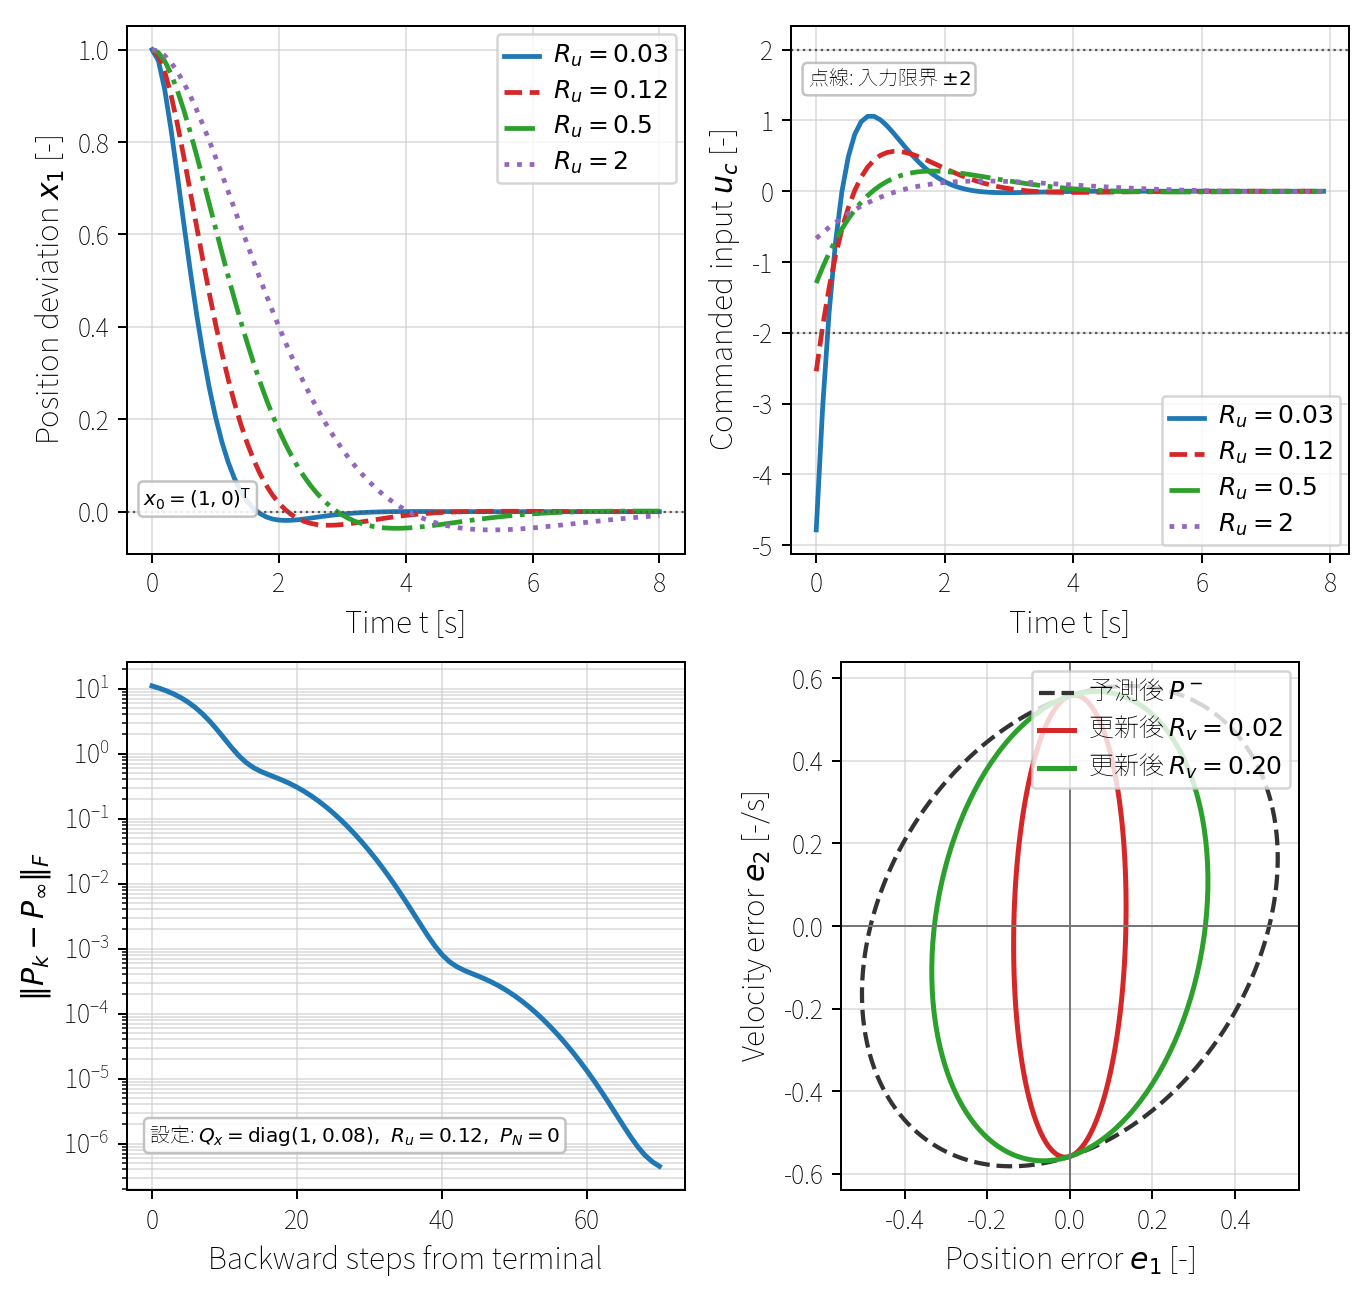
\includegraphics[width=0.95\linewidth,bb=0 0 1368 1296]{figures/lqr_kalman_examples.png}
\caption{二重積分器に対する LQR と Kalman フィルタの調整例。上段は入力重み $R_u$ による状態応答と入力指令の変化であり、入力限界を点線で示している。左下は有限ホライズンの後退リカッチ再帰が定常解へ近づく様子である。右下は予測後の誤差共分散楕円が位置測定によって更新される様子であり、測定ノイズ分散 $R_v$ が小さいほど測定方向の不確かさが強く縮む。}
\label{fig:lqr-kalman-examples}
\end{figure}

左下のリカッチ再帰では、終端条件から後ろ向きに計算した $P_k$ が定常解 $P_\infty$ に近づく。これはホライズンを長くしたとき、現在時刻から十分遠い終端条件の影響が薄れ、無限ホライズン LQR のゲインへ近づくことを表す。右下の共分散楕円は、予測で広がった不確かさが測定更新で縮む過程を示す。位置だけを測っているので、主に位置方向の幅が縮み、速度方向は状態方程式との相関を通じて間接的に修正される。$R_v$ を大きくすると測定を疑うため、更新後楕円は予測楕円に近く残る。

\begin{practice}[重みと共分散図の確認]
図\ref{fig:lqr-kalman-examples}を用いて、$R_u=0.03$ と $R_u=2$ の応答を比較せよ。整定の速さ、最大入力指令、入力限界を越える有無を評価し、実際の入力が飽和する場合に LQR の線形設計と閉ループシミュレーションの結果がずれる理由を説明せよ。さらに右下の共分散楕円について、$R_v$ を大きくしたとき Kalman ゲインが小さくなることを、楕円の縮み方と $K=P^-C^\T(CP^-C^\T+R_v)^{-1}$ から確認せよ。
\end{practice}

\subsection{連続時間 Kalman--Bucy フィルタ}

離散時間 Kalman フィルタでは、時刻 $k-1$ から $k$ へ進める予測と、時刻 $k$ の測定値による更新を分けて書いた。連続時間で測定が絶えず入ってくると考えると、この二段構造は微小時間ごとに連続して繰り返される極限になる。この極限で得られる線形ガウス推定器を Kalman--Bucy フィルタという。

状態を $x(t)\in\R^n$、入力を $u(t)\in\R^m$、測定を $y(t)\in\R^p$ とする。連続時間の線形確率モデルを、白色ノイズを形式的に用いて
\begin{align}
  \dot{x}(t)&=Ax(t)+Bu(t)+Gw(t),\\
  y(t)&=Cx(t)+v(t)
  \label{eq:kb-formal-model}
\end{align}
と書くことが多い。ここで $A\in\R^{n\times n}$、$B\in\R^{n\times m}$、$G\in\R^{n\times r}$、$C\in\R^{p\times n}$ である。$w(t)\in\R^r$ はプロセスノイズ、$v(t)\in\R^p$ は測定ノイズであり、
\begin{align}
  E[w(t)]&=0,
  &E[v(t)]&=0,\\
  E[w(t)w(\tau)^\T]&=Q_w\delta(t-\tau),
  &E[v(t)v(\tau)^\T]&=R_v\delta(t-\tau),\\
  E[w(t)v(\tau)^\T]&=0
\end{align}
を仮定する。$Q_w=Q_w^\T\ge0$ は $r\times r$ のプロセスノイズ強度、$R_v=R_v^\T>0$ は $p\times p$ の測定ノイズ強度である。$\delta(t-\tau)$ は Dirac のデルタであり、連続時間の白色ノイズが普通の関数ではなく、積分したときに有限の分散を持つ理想化であることを表す。

この理想化を少し丁寧に扱うには、独立な Wiener 過程 $\beta(t)\in\R^r$、$\eta(t)\in\R^p$ を用いて
\begin{align}
  \dd x(t)&=(Ax(t)+Bu(t))\,\dd t+G\,\dd\beta(t),\\
  \dd z(t)&=Cx(t)\,\dd t+\dd\eta(t)
  \label{eq:kb-stochastic-model}
\end{align}
と書く。$z(t)$ は測定信号を時間積分した量であり、形式的には $y(t)=\dd z(t)/\dd t$ と見れば \weq{kb-formal-model} に対応する。増分の共分散は
\begin{align}
  E[\dd\beta(t)\dd\beta(t)^\T]&=Q_w\,\dd t,\\
  E[\dd\eta(t)\dd\eta(t)^\T]&=R_v\,\dd t,\\
  E[\dd\beta(t)\dd\eta(t)^\T]&=0
\end{align}
である。以下では、初期推定誤差 $x(0)-\hat{x}(0)$ がこれらのノイズと無相関で、共分散
\begin{equation}
  P(0)=E[(x(0)-\hat{x}(0))(x(0)-\hat{x}(0))^\T]
\end{equation}
を持つとする。

Kalman--Bucy フィルタは、測定の予測誤差を連続時間で注入するオブザーバである。測定微分を用いると
\begin{equation}
  \dd\hat{x}(t)
  =(A\hat{x}(t)+Bu(t))\,\dd t
  +L(t)\{\dd z(t)-C\hat{x}(t)\,\dd t\}
  \label{eq:kb-filter-differential}
\end{equation}
であり、形式的な測定 $y(t)$ を用いれば
\begin{equation}
  \dot{\hat{x}}(t)
  =A\hat{x}(t)+Bu(t)+L(t)\{y(t)-C\hat{x}(t)\}
  \label{eq:kb-filter-formal}
\end{equation}
と書ける。$L(t)\in\R^{n\times p}$ は連続時間の Kalman ゲインである。$y-C\hat{x}$ は離散時間の場合の革新 $\nu_k=y_k-C_k\hat{x}_{k|k-1}$ に対応し、測定が予測より大きい方向へ状態推定を修正する信号である。

\begin{derivation}
推定誤差を
\begin{equation}
  e(t)=x(t)-\hat{x}(t)
\end{equation}
と置く。\weq{kb-stochastic-model} と \weq{kb-filter-differential} の差を取ると
\begin{align}
  \dd e
  &=\dd x-\dd\hat{x}\\
  &=(Ax+Bu)\,\dd t+G\,\dd\beta
    -(A\hat{x}+Bu)\,\dd t
    -L\{C(x-\hat{x})\,\dd t+\dd\eta\}\\
  &=(A-LC)e\,\dd t+G\,\dd\beta-L\,\dd\eta
  \label{eq:kb-error-dynamics}
\end{align}
を得る。入力 $u$ は既知として推定器にも入っているため、誤差方程式から消える。

誤差共分散を
\begin{equation}
  P(t)=E[e(t)e(t)^\T]\in\R^{n\times n}
\end{equation}
と定義する。微小変化では積の微分に二次のノイズ増分が残るので、Itô の積公式
\begin{equation}
  \dd(ee^\T)=(\dd e)e^\T+e(\dd e)^\T+(\dd e)(\dd e)^\T
\end{equation}
を使う。\weq{kb-error-dynamics} を代入して期待値を取ると、$e$ と新しいノイズ増分の交差項、および $\dd\beta$ と $\dd\eta$ の交差項は仮定により消える。残る項は
\begin{align}
  \dot{P}
  &=(A-LC)P+P(A-LC)^\T
    +GQ_wG^\T+LR_vL^\T\\
  &=AP+PA^\T+GQ_wG^\T
    -LCP-PC^\T L^\T+LR_vL^\T.
  \label{eq:kb-covariance-for-gain}
\end{align}
ここで $GQ_wG^\T$ はプロセスノイズが状態共分散を増やす項、$LR_vL^\T$ は測定ノイズをゲインで状態空間へ戻した項である。一方で $-LCP-PC^\T L^\T$ は、測定から得た情報が推定誤差を減らす効果を表す。

離散時間の場合と同じく、瞬間的な共分散の増え方を小さくする $L$ を選ぶ。記号を軽くするため $R=R_v$ と書くと、$L$ に依存する部分は
\begin{equation}
  -LCP-PC^\T L^\T+LRL^\T
\end{equation}
である。これを平方完成すると
\begin{align}
  -LCP-PC^\T L^\T+LRL^\T
  &=
  (L-PC^\T R^{-1})R(L-PC^\T R^{-1})^\T\\
  &\quad -PC^\T R^{-1}CP.
\end{align}
$R_v>0$ なので第一項は半正定値であり、最小にするゲインは
\begin{equation}
  L(t)=P(t)C^\T R_v^{-1}
  \label{eq:kb-gain}
\end{equation}
である。これを \weq{kb-covariance-for-gain} に代入すると、連続時間 Kalman--Bucy フィルタの共分散リカッチ方程式
\begin{equation}
  \dot{P}
  =AP+PA^\T+GQ_wG^\T
  -PC^\T R_v^{-1}CP,
  \qquad P(0)=P_0
  \label{eq:kb-riccati}
\end{equation}
を得る。
\end{derivation}

\weq{kb-riccati} は LQR のリカッチ方程式とよく似ている。LQR では入力を使って状態の増大を抑えるために $-PBR^{-1}B^\T P$ が現れた。Kalman--Bucy フィルタでは測定を使って推定誤差を抑えるために $-PC^\T R_v^{-1}CP$ が現れる。$GQ_wG^\T$ はモデルをどれだけ疑うか、$R_v$ は測定をどれだけ疑うかを表す。$Q_w$ を大きくすれば $P$ が大きくなりやすく、ゲイン $L=PC^\T R_v^{-1}$ は測定へ強く反応する。$R_v$ を大きくすれば、測定の信頼度が下がり、ゲインは小さくなる。

時不変で長時間運転する場合、条件がよければ $P(t)$ は定常値 $P_\infty$ に収束する。このとき
\begin{equation}
  0=AP_\infty+P_\infty A^\T+GQ_wG^\T
  -P_\infty C^\T R_v^{-1}CP_\infty
\end{equation}
を満たし、定常ゲインは
\begin{equation}
  L_\infty=P_\infty C^\T R_v^{-1}
\end{equation}
である。代表的な十分条件は、測定から不安定なモードを観測できるという可検出性と、プロセスノイズで励起される不確かさが安定化可能な範囲にあることである。すなわち、推定すべき不安定な動きが測定にまったく現れなければ、どれだけゲインを調整しても誤差を抑えられない。

離散時間 Kalman フィルタとの対応は、微小時間幅 $h$ で見ると分かりやすい。測定を無視してモデルだけで進めれば
\begin{align}
  \hat{x}(t+h)&=\hat{x}(t)+h(A\hat{x}(t)+Bu(t))+O(h^2),\\
  P(t+h)&=P(t)+h\{AP(t)+P(t)A^\T+GQ_wG^\T\}+O(h^2)
\end{align}
となり、これは離散時間の予測ステップに対応する。一方、同じ微小時間内に入る連続測定は、共分散を
\begin{equation}
  -h\,P(t)C^\T R_v^{-1}CP(t)
\end{equation}
だけ減らす方向に働く。したがって、離散時間の「予測してから更新する」という二段階は、連続時間では一つの微分方程式の中で同時に進む。数値実装では、\weq{kb-filter-differential} と \weq{kb-riccati} を時間刻みで積分するか、サンプリング周期 $h$ ごとに
\begin{align}
  A_d&=e^{Ah},\\
  B_d&=\int_0^h e^{A\sigma}B\,\dd\sigma,\\
  Q_d&=\int_0^h e^{A\sigma}GQ_wG^\T e^{A^\T\sigma}\,\dd\sigma
\end{align}
を用いて離散時間モデルへ変換し、前節の離散時間 Kalman フィルタを使う。

実用上は、連続時間の白色ノイズをそのまま物理信号と見なしてはいけない。白色ノイズは全周波数に同じ強度を持つ理想化であり、実際の外乱やセンサノイズには帯域、遅れ、量子化、フィルタ処理がある。また、サンプルされたセンサ値の分散 $R_s$ と、連続時間モデルの強度 $R_v$ は同じ量ではない。測定が区間平均なのか、瞬時値をサンプルしたものなのか、前段のアナログフィルタを通っているのかによって対応が変わる。連続モデルから実装へ移すときは、サンプリング周期、ノイズ強度の単位、離散化した $Q_d$ と測定共分散の意味をそろえる必要がある。熱系の温度推定のような低速の対象でも、モデル化していない熱流を $Q_w$ で表すのか、センサ読み取りのばらつきを $R_v$ または離散時間の $R_s$ で表すのかを分けて調整することが、フィルタの応答を評価する第一条件になる。

\subsection{LQG 制御と分離原理}

LQR は状態 $x$ が利用できるときの二次評価最適な入力を与え、Kalman フィルタは測定 $y$ から状態の条件付き平均を推定する。多くの制御対象では、速度、内部温度、ばねの伸び、電流の一部などが直接測れないため、状態フィードバック $u=-Kx$ はそのまま実装できない。そこで、測れる出力から $\hat{x}$ を作り、状態フィードバックの $x$ を $\hat{x}$ で置き換える。この構成を、線形二次ガウス制御、すなわち LQG 制御という。名称の Linear はモデルが線形であること、Quadratic は評価関数が二次形式であること、Gaussian はノイズと初期状態の確率モデルを正規分布で扱うことを表している。

連続時間の標準的な LQG 問題を
\begin{align}
  \dot{x}(t)&=Ax(t)+Bu(t)+Gw(t),\\
  y(t)&=Cx(t)+v(t)
  \label{eq:lqg-plant}
\end{align}
と置く。状態は $x\in\R^n$、入力は $u\in\R^m$、測定は $y\in\R^p$ である。$w$ はモデル化しない外乱や入力されない揺らぎを表すプロセスノイズ、$v$ は測定ノイズである。ここでは
\begin{align}
  E[w(t)]&=0,
  &E[v(t)]&=0,\\
  E[w(t)w(\tau)^\T]&=Q_w\delta(t-\tau),
  &E[v(t)v(\tau)^\T]&=R_v\delta(t-\tau),\\
  E[w(t)v(\tau)^\T]&=0
\end{align}
を仮定し、$Q_w=Q_w^\T\ge0$、$R_v=R_v^\T>0$ とする。初期状態の推定誤差も、これらのノイズと無相関であると仮定する。制御性能は、有限ホライズンなら
\begin{equation}
  J_T
  =E\left[
    x(T)^\T S x(T)
    +\int_0^T
      \{x(t)^\T Q_x x(t)+u(t)^\T R_u u(t)\}\,\dd t
  \right]
  \label{eq:lqg-finite-cost}
\end{equation}
で評価する。ここで $Q_x=Q_x^\T\ge0$、$R_u=R_u^\T>0$、$S=S^\T\ge0$ であり、$Q_x$ は状態偏差への重み、$R_u$ は入力への重みである。プロセスノイズが持続的に入る無限ホライズンでは、単純な積分型の期待コストは一般に時間とともに増え続けるため、定常運転の評価には
\begin{equation}
  \bar{J}
  =
  \limsup_{T\to\infty}
  \frac{1}{T}
  E\int_0^T
    \{x(t)^\T Q_x x(t)+u(t)^\T R_u u(t)\}\,\dd t
  \label{eq:lqg-average-cost}
\end{equation}
のような平均コストを用いる。初期値だけを減衰させる決定論的 LQR と、持続的なノイズを受ける LQG では、この点で評価の意味が異なる。

LQG の制御器は、制御用リカッチ方程式と推定用リカッチ方程式を別々に解いて作る。有限ホライズンの制御側では
\begin{equation}
  -\dot{P}_c
  =
  A^\T P_c+P_cA-P_cBR_u^{-1}B^\T P_c+Q_x,
  \qquad
  P_c(T)=S
  \label{eq:lqg-control-rde}
\end{equation}
を解き、
\begin{equation}
  K(t)=R_u^{-1}B^\T P_c(t)
  \label{eq:lqg-control-gain}
\end{equation}
とする。無限ホライズンで定常ゲインを使う場合は、対応する代数リカッチ方程式
\begin{equation}
  A^\T P_c+P_cA-P_cBR_u^{-1}B^\T P_c+Q_x=0
  \label{eq:lqg-control-care}
\end{equation}
の安定化解から $K=R_u^{-1}B^\T P_c$ を得る。一方、推定側では Kalman--Bucy フィルタの共分散リカッチ方程式
\begin{equation}
  \dot{P}_e
  =
  AP_e+P_eA^\T+GQ_wG^\T
  -P_eC^\T R_v^{-1}CP_e
  \label{eq:lqg-estimator-rde}
\end{equation}
を用い、
\begin{equation}
  L(t)=P_e(t)C^\T R_v^{-1}
  \label{eq:lqg-estimator-gain}
\end{equation}
とする。定常推定器では
\begin{equation}
  0=
  AP_e+P_eA^\T+GQ_wG^\T
  -P_eC^\T R_v^{-1}CP_e
  \label{eq:lqg-estimator-care}
\end{equation}
の安定化解を使う。制御側の $P_c$ は将来の制御コストを表し、推定側の $P_e$ は推定誤差の共分散を表す。同じリカッチ方程式という名前で呼ばれても、二つの行列が表す量は異なる。

得られた LQG 制御器は
\begin{align}
  \dot{\hat{x}}&=A\hat{x}+Bu+L(y-C\hat{x}),\\
  u&=-K\hat{x}
  \label{eq:lqg-controller}
\end{align}
である。$y-C\hat{x}$ は測定の革新であり、推定器はこの革新を用いて $\hat{x}$ を修正する。制御入力は、推定値 $\hat{x}$ を真の状態であるかのように扱って LQR ゲインを掛ける。この性質を確定性等価性という。確定性等価性は、「不確かさを無視してよい」という意味ではない。ノイズ共分散は推定器の $L$ を決め、推定誤差は閉ループの入力変動や状態変動として現れる。ただし、最適な制御則の形は、完全状態が測れる LQR の $x$ を条件付き平均 $\hat{x}$ に置き換えたものになる。

図\ref{fig:lqg-signal-path}は、この式を信号経路として並べたものである。制御器が計算する信号を入力指令 $u_c=-K\hat{x}$、アクチュエータを通って対象へ実際に入る信号を $u_a$ と区別している。線形 LQG の導出では $u_a=u_c$ を仮定するが、飽和やレート制限が入る実装では $u_a$ が推定器にも渡される既知入力でなければならない。推定器が $u_c$ を使い続けると、対象に入った入力との不一致が推定誤差として蓄積し、分離原理の前提から外れる。

\begin{figure}[tb]
\centering
\setlength{\unitlength}{1mm}
\begin{picture}(136,68)
\small
\put(16,44){\framebox(34,12){\shortstack{制御器\\$u_c=-K\hat{x}$}}}
\put(58,44){\framebox(30,12){\shortstack{飽和・駆動\\$u_a$}}}
\put(98,44){\framebox(28,12){\shortstack{対象\\$x$}}}
\put(98,14){\framebox(28,12){\shortstack{測定\\$y=Cx+v$}}}
\put(16,14){\framebox(34,12){\shortstack{推定器\\$\hat{x}$}}}
\put(50,50){\vector(1,0){8}}
\put(51,53){$u_c$}
\put(88,50){\vector(1,0){10}}
\put(90,53){$u_a$}
\put(112,65){\vector(0,-1){9}}
\put(114,60){$w$}
\put(112,44){\vector(0,-1){18}}
\put(115,35){$x$}
\put(132,20){\vector(-1,0){6}}
\put(129,22){$v$}
\put(98,20){\vector(-1,0){48}}
\put(74,22){$y$}
\put(33,26){\vector(0,1){18}}
\put(35,34){$\hat{x}$}
\put(73,44){\line(0,-1){12}}
\put(73,32){\vector(-1,0){28}}
\put(45,32){\vector(0,-1){6}}
\put(50,34){既知入力 $u_a$}
\end{picture}
\caption{LQG 制御の信号経路。測定 $y$ から推定器が $\hat{x}$ を作り、制御器が入力指令 $u_c$ を計算し、飽和や駆動系を通った実入力 $u_a$ が対象へ入る。線形導出では $u_a=u_c$ とみなすが、飽和がある場合は実入力を推定器の既知入力として扱う。}
\label{fig:lqg-signal-path}
\end{figure}

この置き換えが成立する理由は、条件付き平均と推定誤差の直交性にある。時刻 $t$ までの測定履歴を $\mathcal{Y}_t$ とし、
\begin{equation}
  \hat{x}(t)=E[x(t)\mid\mathcal{Y}_t],
  \qquad
  e(t)=x(t)-\hat{x}(t)
\end{equation}
と置く。条件付き平均の定義より
\begin{equation}
  E[e(t)\mid\mathcal{Y}_t]=0
\end{equation}
である。したがって、状態重みの条件付き期待値は
\begin{align}
  E[x^\T Q_x x\mid\mathcal{Y}_t]
  &=
  E[(\hat{x}+e)^\T Q_x(\hat{x}+e)\mid\mathcal{Y}_t]\\
  &=
  \hat{x}^\T Q_x\hat{x}
  +2\hat{x}^\T Q_x E[e\mid\mathcal{Y}_t]
  +E[e^\T Q_x e\mid\mathcal{Y}_t]\\
  &=
  \hat{x}^\T Q_x\hat{x}
  +\tr(Q_xP_e(t)).
  \label{eq:lqg-cost-decomposition}
\end{align}
最後の等号では $P_e(t)=E[ee^\T\mid\mathcal{Y}_t]$ と、$E[e^\T Q_x e]=\tr(Q_x E[ee^\T])$ を使った。右辺の第一項だけが、現在の推定値を状態として見た LQR の状態コストである。第二項は推定誤差から避けられずに生じるコストであり、線形ガウスモデルと既知入力の仮定のもとでは、推定誤差共分散の時間発展は制御入力の選び方に依存しない。入力コスト $u^\T R_u u$ はそのまま制御側に残るので、制御の最適化は $\hat{x}$ を状態とする LQR と同じ形になる。これが LQG における分離原理の中身である。

\begin{theorem}[LQG の分離原理]
線形モデル \weq{lqg-plant}、二次評価 \weq{lqg-finite-cost}、ゼロ平均の独立なガウスノイズ、既知入力、および初期推定誤差とノイズの独立性を仮定する。制御側リカッチ方程式と推定側リカッチ方程式がそれぞれ適切な解を持つなら、最適な出力フィードバック制御器は Kalman フィルタと LQR 状態フィードバックを
\begin{equation}
  u(t)=-K(t)\hat{x}(t)
\end{equation}
で直列に接続した形で与えられる。定常無限ホライズンでは、$(A,B)$ の可安定性、$(A,Q_x^{1/2})$ の可検出性、$(A,C)$ の可検出性、および $W=GQ_wG^\T$ に対する $(A,W^{1/2})$ の可安定性が代表的な十分条件である。
\end{theorem}

分離原理という名前は、閉ループの状態方程式にも直接現れる。推定誤差を
\begin{equation}
  e=x-\hat{x}
\end{equation}
と置き、定常ゲイン $K,L$ を用いると
\begin{align}
  \dot{x}
  &=Ax+B(-K\hat{x})+Gw\\
  &=(A-BK)x+BKe+Gw,
\end{align}
であり、推定誤差は
\begin{align}
  \dot{e}
  &=\dot{x}-\dot{\hat{x}}\\
  &=(A-LC)e+Gw-Lv
\end{align}
を満たす。したがって、拡大状態 $(x,e)$ に対する閉ループは
\begin{equation}
  \begin{bmatrix}
    \dot{x}\\
    \dot{e}
  \end{bmatrix}
  =
  \begin{bmatrix}
    A-BK & BK\\
    0 & A-LC
  \end{bmatrix}
  \begin{bmatrix}
    x\\
    e
  \end{bmatrix}
  +
  \begin{bmatrix}
    G & 0\\
    G & -L
  \end{bmatrix}
  \begin{bmatrix}
    w\\
    v
  \end{bmatrix}.
  \label{eq:lqg-augmented-dynamics}
\end{equation}
係数行列はブロック上三角である。ノイズを 0 として平均の安定性だけを見ると、その固有値は $A-BK$ の固有値と $A-LC$ の固有値を合わせたものになる。したがって、LQR で $A-BK$ を Hurwitz にし、Kalman--Bucy フィルタで $A-LC$ を Hurwitz にすれば、平均的な閉ループは安定になる。さらにノイズ強度が有限で、両方の行列が Hurwitz なら、拡大系の共分散も定常値へ収束し、状態と推定誤差の二乗平均は有界に保たれる。

調整の解釈は二組に分けると整理しやすい。$Q_x$ と $R_u$ は、制御として何を優先するかを決める。$Q_x$ を大きくすると状態偏差を強く抑えるため $K$ が大きくなりやすく、応答は速くなる一方で入力の振れや飽和の危険が増える。$R_u$ を大きくすると入力を節約し、応答は穏やかになる。これに対し、$Q_w$ と $R_v$ は、推定器がモデルと測定のどちらを信じるかを決める。$Q_w$ を大きくすると、モデル化しない外乱が大きいと見なされ、推定器は測定の革新へ強く反応する。$R_v$ を大きくすると、測定値を疑うため $L$ は小さくなり、推定値はモデル予測に近づく。たとえば熱系で室温を制御する場合、外気や人の出入りによる未モデル化熱流が大きいなら $Q_w$ を増やし、温度センサのばらつきや量子化が大きいなら $R_v$ を増やす。入力重み $R_u$ はヒータ出力の制限や消費電力に対応し、状態重み $Q_x$ は温度偏差をどれだけ早く戻したいかに対応する。

ただし、分離して設計できることと、相互作用を確認しなくてよいことは同じではない。$K$ が大きいと、推定値に含まれる高周波の測定ノイズ成分が入力へ強く入る。$L$ が大きいと、推定値は測定に素早く追従するが、センサノイズにも敏感になる。入力飽和、レート制限、むだ時間、非線形性、モデル誤差、ノイズの相関、非ガウス分布、センサの帯域制限があると、上の分離原理の仮定から外れる。特に入力が飽和すると、推定器が仮定している既知入力 $u$ と実際に対象へ入った入力がずれ、推定誤差の独立なリカッチ方程式という構造が崩れる。LQG は線形ガウスモデルに対する基準設計として強力であるが、最終的な設計では飽和を含む閉ループシミュレーション、ノイズ共分散の妥当性確認、革新系列の白色性、入力の実効範囲、モデル誤差に対する感度を確認する必要がある。

離散時間でも同じ構造が成り立つ。離散時間 LQR のリカッチ方程式から $K_k$ を求め、離散時間 Kalman フィルタから $\hat{x}_{k|k}$ を求めて
\begin{equation}
  u_k=-K_k\hat{x}_{k|k}
\end{equation}
とすればよい。実装では、サンプリング周期、ゼロ次ホールドで離散化した $A_d,B_d,Q_d$、測定時刻、計算遅れをそろえる。連続時間の式で設計したゲインをそのままデジタル制御器へ入れるのではなく、実際のサンプル周期で推定と制御がどの順序で実行されるかを明示することが、LQG を実機へ移すときの第一条件である。

\subsection{固定区間平滑化と RTS 平滑化}

Kalman フィルタの推定値 $\hat{x}_{k|k}$ は、時刻 $k$ までの測定履歴 $\mathcal{Y}_k$ を使った推定である。実時間制御では未来の測定値を待てないため、この片方向の推定が自然である。一方、実験後のデータ解析、軌道再構成、パラメータ同定、センサログの補正では、区間全体の測定値
\begin{equation}
  \mathcal{Y}_N=\{y_0,y_1,\ldots,y_N\}
\end{equation}
がすでに手元にある。このとき、時刻 $k<N$ の状態を推定するために $y_{k+1},\ldots,y_N$ も使える。区間 $0,\ldots,N$ 全体の測定値を用いて $x_k$ を推定する処理を固定区間平滑化という。表記として
\begin{equation}
  \hat{x}_{k|N}=E[x_k\mid\mathcal{Y}_N],
  \qquad
  P_{k|N}=E[(x_k-\hat{x}_{k|N})(x_k-\hat{x}_{k|N})^\T\mid\mathcal{Y}_N]
\end{equation}
を用いる。

平滑化はフィルタリングの否定ではなく、フィルタリングに未来側の情報を後から戻す操作である。熱系で例えれば、時刻 $k$ の温度推定は、その時刻までのセンサ値だけでなく、その後の温度の上がり方や下がり方からも制約を受ける。後で温度が急に上がったなら、時刻 $k$ の未モデル化熱流がすでに始まっていた可能性が高い。固定区間平滑化は、このような「後で分かった整合条件」をモデルの時間発展を通じて過去へ伝える。

代表的な線形ガウス平滑化が Rauch--Tung--Striebel 平滑化、すなわち RTS 平滑化である。離散時間モデルを
\begin{equation}
  x_{k+1}=A_kx_k+B_ku_k+G_kw_k
\end{equation}
とし、前向きの Kalman フィルタで
\begin{equation}
  \hat{x}_{k|k},
  \quad
  P_{k|k},
  \quad
  \hat{x}_{k+1|k},
  \quad
  P_{k+1|k}
\end{equation}
を保存しておく。ここで
\begin{align}
  \hat{x}_{k+1|k}
  &=A_k\hat{x}_{k|k}+B_ku_k,\\
  P_{k+1|k}
  &=A_kP_{k|k}A_k^\T+G_kQ_{w,k}G_k^\T
\end{align}
である。終端では、未来の測定値がもうないので
\begin{equation}
  \hat{x}_{N|N}
  \quad\text{と}\quad
  P_{N|N}
\end{equation}
をそのまま平滑化の初期値として用いる。すなわち
\begin{equation}
  \hat{x}_{N|N}^{\mathrm{s}}=\hat{x}_{N|N},
  \qquad
  P_{N|N}^{\mathrm{s}}=P_{N|N}
\end{equation}
と書く。ただし上付き $\mathrm{s}$ は平滑化後の量を表す記号であり、以下では
\begin{equation}
  \hat{x}_{k|N}=\hat{x}_{k|N}^{\mathrm{s}},
  \qquad
  P_{k|N}=P_{k|N}^{\mathrm{s}}
\end{equation}
と同じ意味で使う。

RTS 平滑化では、$k=N-1,N-2,\ldots,0$ と時間を逆向きに進める。平滑化ゲインを
\begin{equation}
  J_k=P_{k|k}A_k^\T P_{k+1|k}^{-1}
  \label{eq:rts-smoother-gain}
\end{equation}
と置くと、平均と共分散は
\begin{align}
  \hat{x}_{k|N}
  &=
  \hat{x}_{k|k}
  +J_k(\hat{x}_{k+1|N}-\hat{x}_{k+1|k}),
  \label{eq:rts-smoother-mean}\\
  P_{k|N}
  &=
  P_{k|k}
  +J_k(P_{k+1|N}-P_{k+1|k})J_k^\T
  \label{eq:rts-smoother-covariance}
\end{align}
で更新される。\weq{rts-smoother-mean} の括弧
\begin{equation}
  \hat{x}_{k+1|N}-\hat{x}_{k+1|k}
\end{equation}
は、時刻 $k+1$ の状態について、未来の測定値を含めた推定が前向き予測からどれだけずれたかを表す。このずれを、$x_k$ と $x_{k+1}$ の相関を表す係数 $J_k$ で時刻 $k$ へ戻す。共分散式 \weq{rts-smoother-covariance} では、未来の測定値を使うことで $P_{k+1|N}$ が通常 $P_{k+1|k}$ より小さくなるため、その減少分が $J_k$ を通じて $P_{k|k}$ から差し引かれる。

\weq{rts-smoother-gain} は逆行列を明示しているが、実装では $P_{k+1|k}^{-1}$ を直接作らない。線形方程式
\begin{equation}
  P_{k+1|k}X^\T=A_kP_{k|k}
\end{equation}
を Cholesky 分解や対称正定値用の解法で解き、$J_k=X$ とする。$P_{k+1|k}$ が特異に近い場合は、プロセスノイズの設定、モデルの可観測性、状態の単位スケーリングを見直す必要がある。平滑化は未来情報を使うため、実時間フィードバック制御器の中にはそのまま入れられない。固定遅れ平滑化のように数サンプルだけ遅らせる実装もあるが、遅れを許せない制御ループでは、平滑化は主にログ解析や推定器調整のための手段になる。

\subsection{情報形式の Kalman フィルタ}

共分散形式の Kalman フィルタは、推定誤差共分散 $P$ と推定平均 $\hat{x}$ を主変数にする。これに対して、情報形式の Kalman フィルタは
\begin{equation}
  Y=P^{-1},
  \qquad
  \eta=Y\hat{x}
  \label{eq:information-state}
\end{equation}
を主変数にする。$Y$ を情報行列、$\eta$ を情報ベクトルという。$P$ が大きいことは不確かさが大きいことを意味するので、その逆行列 $Y$ は状態についてどれだけ情報を持っているかを表す。推定値そのものは
\begin{equation}
  \hat{x}=Y^{-1}\eta
\end{equation}
で戻せるが、数値実装ではこの逆行列も直接作らず、線形方程式
\begin{equation}
  Y\hat{x}=\eta
\end{equation}
を解く。

情報形式の利点は、測定更新が加算で書けることである。時刻 $k$ の予測情報を $Y_{k|k-1}$、$\eta_{k|k-1}$ とし、測定モデルを
\begin{equation}
  y_k=C_kx_k+v_k,
  \qquad
  v_k\sim(0,R_{v,k})
\end{equation}
とする。測定を得た後の情報行列と情報ベクトルは
\begin{align}
  Y_{k|k}
  &=
  Y_{k|k-1}+C_k^\T R_{v,k}^{-1}C_k,
  \label{eq:information-update-matrix}\\
  \eta_{k|k}
  &=
  \eta_{k|k-1}+C_k^\T R_{v,k}^{-1}y_k.
  \label{eq:information-update-vector}
\end{align}
この式は、ガウス分布の指数部を足し合わせるだけで導ける。予測分布が
\begin{equation}
  p(x_k\mid\mathcal{Y}_{k-1})
  \propto
  \exp\left[
    -\frac{1}{2}x_k^\T Y_{k|k-1}x_k
    +\eta_{k|k-1}^\T x_k
  \right]
\end{equation}
であり、測定尤度が
\begin{equation}
  p(y_k\mid x_k)
  \propto
  \exp\left[
    -\frac{1}{2}(y_k-C_kx_k)^\T R_{v,k}^{-1}(y_k-C_kx_k)
  \right]
\end{equation}
であるとする。$x_k$ に依存する項だけを集めると
\begin{align}
  &-\frac{1}{2}x_k^\T Y_{k|k-1}x_k+\eta_{k|k-1}^\T x_k\\
  &\quad
  -\frac{1}{2}x_k^\T C_k^\T R_{v,k}^{-1}C_kx_k
  +x_k^\T C_k^\T R_{v,k}^{-1}y_k
\end{align}
となる。二次項の係数と一次項の係数を読み取れば、\weq{information-update-matrix} と \weq{information-update-vector} が得られる。測定値だけに依存する定数項は正規化定数に吸収される。

複数の独立なセンサが同じ時刻に入る場合、この加算性はさらに明確になる。センサ $i$ が
\begin{equation}
  y_k^{(i)}=C_k^{(i)}x_k+v_k^{(i)},
  \qquad
  E[v_k^{(i)}(v_k^{(j)})^\T]=0\quad(i\ne j)
\end{equation}
を満たすなら、
\begin{align}
  Y_{k|k}
  &=
  Y_{k|k-1}
  +\sum_i (C_k^{(i)})^\T
    (R_{v,k}^{(i)})^{-1}C_k^{(i)},\\
  \eta_{k|k}
  &=
  \eta_{k|k-1}
  +\sum_i (C_k^{(i)})^\T
    (R_{v,k}^{(i)})^{-1}y_k^{(i)}
\end{align}
でよい。したがって、センサが非同期に届く場合でも、その測定に対応する情報だけを順に足せる。$C_k^{(i)}$ が状態ベクトルの一部だけを見る疎な行列であれば、各センサが加える情報行列も疎になる。大規模な温度場、電力網、移動体群、SLAM のように、全状態のうち局所的な組だけを各測定が結びつける問題では、共分散行列 $P$ が密になりやすい一方で、情報行列 $Y$ やその Cholesky 因子は疎構造を保てることがある。この性質により、疎行列用の順序付け、疎 Cholesky 分解、局所測定の逐次追加が使いやすくなる。

時間予測は、測定更新ほど単純な加算にはならない。線形モデル
\begin{equation}
  x_k=A_{k-1}x_{k-1}+B_{k-1}u_{k-1}+q_{k-1},
  \qquad
  q_{k-1}\sim(0,Q_{k-1})
\end{equation}
を用いるなら、共分散形式では
\begin{align}
  \hat{x}_{k|k-1}
  &=A_{k-1}\hat{x}_{k-1|k-1}+B_{k-1}u_{k-1},\\
  P_{k|k-1}
  &=A_{k-1}P_{k-1|k-1}A_{k-1}^\T+Q_{k-1}
\end{align}
を計算してから
\begin{equation}
  Y_{k|k-1}=P_{k|k-1}^{-1},
  \qquad
  \eta_{k|k-1}=Y_{k|k-1}\hat{x}_{k|k-1}
  \label{eq:information-prediction-vector}
\end{equation}
とすればよい。ここでも $\hat{x}_{k|k-1}=Y_{k|k-1}^{-1}\eta_{k|k-1}$ を取り出す場面では逆行列を明示的に作らず、線形方程式 $Y_{k|k-1}\hat{x}_{k|k-1}=\eta_{k|k-1}$ を解く。情報形式だけで表す場合も Woodbury の公式により
\begin{equation}
  Y_{k|k-1}
  =
  Q_{k-1}^{-1}
  -Q_{k-1}^{-1}A_{k-1}
  (Y_{k-1|k-1}+A_{k-1}^\T Q_{k-1}^{-1}A_{k-1})^{-1}
  A_{k-1}^\T Q_{k-1}^{-1}
  \label{eq:information-prediction-matrix}
\end{equation}
と書ける。ただし、この式は $Q_{k-1}$ が正定値であることを仮定しており、数値的には内側の線形方程式を疎分解で解く形で実装する。入力 $B_{k-1}u_{k-1}$ は平均を平行移動する項なので、情報ベクトルの予測では予測平均を通じて反映される。実装上は、予測段階を共分散形式または平方根形式で行い、測定更新だけを情報形式で疎に処理する混合構成も多い。重要なのは、どの形式でも同じ条件付きガウス分布を表しており、問題の疎性、センサ数、必要な出力が平均なのか共分散なのかに応じて表現を選ぶことである。

\subsection{数値安定性を保つ Kalman フィルタ実装}

Kalman フィルタの式は短いが、有限精度計算では共分散行列の対称性、半正定値性、条件数を保つことが設計の一部になる。共分散 $P$ は本来
\begin{equation}
  P=P^\T,
  \qquad
  z^\T Pz\ge0\quad(\forall z)
\end{equation}
を満たす。しかし、簡略形
\begin{equation}
  P_{k|k}=(I-K_kC_k)P_{k|k-1}
\end{equation}
をそのまま浮動小数点で計算すると、丸め誤差により $P_{k|k}$ がわずかに非対称になったり、負の固有値を持ったりすることがある。負の分散は確率モデルとして意味を持たず、次の Cholesky 分解やゲイン計算を破綻させる。

第一の実装原則は、共分散更新に Joseph 形式を使うことである。
\begin{equation}
  P_{k|k}
  =(I-K_kC_k)P_{k|k-1}(I-K_kC_k)^\T+K_kR_{v,k}K_k^\T
  \label{eq:stable-joseph-form}
\end{equation}
右辺は、半正定値行列を左右から掛けた項と、測定ノイズ共分散をゲインで写した項の和である。したがって、$P_{k|k-1}\ge0$、$R_{v,k}>0$ なら、数学的には $P_{k|k}\ge0$ が保たれる。簡略形と代数的には同じでも、Joseph 形式は丸め誤差に対して共分散の構造を壊しにくい。

第二の原則は、逆行列を明示的に作らないことである。Kalman ゲインを
\begin{equation}
  K_k=P_{k|k-1}C_k^\T S_k^{-1},
  \qquad
  S_k=C_kP_{k|k-1}C_k^\T+R_{v,k}
\end{equation}
と書いても、実装では $S_k^{-1}$ を計算しない。$S_k$ が対称正定値なら Cholesky 分解
\begin{equation}
  S_k=L_kL_k^\T
\end{equation}
を行い、三角行列の連立一次方程式を二回解いて $K_k$ を得る。$S_k$ の Cholesky 分解が失敗する場合、測定ノイズ共分散 $R_{v,k}$ が正定値になっていない、$P_{k|k-1}$ の半正定値性が崩れている、または状態や測定のスケーリングが悪い可能性がある。

第三の原則は、平方根形式を使って共分散そのものではなく因子を更新することである。たとえば
\begin{equation}
  P_{k|k}=S_{k|k}S_{k|k}^\T
\end{equation}
を保ちながら、$S_{k|k}$ を QR 分解や Cholesky 更新で計算する。予測段階では、行列
\begin{equation}
  \begin{bmatrix}
    A_{k-1}S_{k-1|k-1} & G_{k-1}Q_{w,k-1}^{1/2}
  \end{bmatrix}
\end{equation}
の積から $P_{k|k-1}$ を作る代わりに、この横長行列の転置に QR 分解を適用して $S_{k|k-1}$ を得る。測定更新でも、革新共分散や事後共分散の平方根を QR 分解で更新できる。平方根形式では、半正定値性が因子の積として表されるため、丸め誤差で小さな負の固有値が出る危険が減る。情報形式でも同様に
\begin{equation}
  Y_{k|k}=R_{k|k}^\T R_{k|k}
\end{equation}
のような平方根情報形式を使えば、疎 Cholesky 分解と相性がよい。

第四の原則は、対称化と条件数の監視を明示的に行うことである。計算後の共分散は
\begin{equation}
  P\leftarrow\frac{1}{2}(P+P^\T)
\end{equation}
で対称化してから次のステップへ渡すと、丸めによる反対称成分を抑えられる。さらに、$Q_w$、$R_v$、$P_0$ は対称行列として入力し、必要なら
\begin{equation}
  Q_w\leftarrow\frac{1}{2}(Q_w+Q_w^\T),
  \qquad
  R_v\leftarrow\frac{1}{2}(R_v+R_v^\T)
\end{equation}
と確認する。$R_v$ は通常正定値であるべきなので、分散が 0 に近い測定を完全に信じる設定は避け、小さな正の下限を置く。$Q_w$ は半正定値でもよいが、モデルが実際より硬すぎると $P$ が過小になり、革新に対して不自然に鈍い推定器になる。共分散の固有値を無理に切り上げる処理は最後の保護としては使えるが、それを常用しなければ動かない場合は、ノイズ共分散、離散化、単位スケーリング、観測モデルのいずれかを見直すべきである。

状態のスケーリングも数値安定性に直結する。位置をメートル、角度をラジアン、温度を摂氏、電流をアンペアで混在させること自体は自然だが、それらの典型値が $10^{-6}$ と $10^6$ のように大きく離れると、$P$ や $S_k$ の条件数が悪くなる。状態を無次元化する、代表値で割って同程度の大きさにする、重みや共分散をそのスケールに合わせて変換する、といった処理は、理論式を変えるのではなく、同じ推定問題を計算しやすい座標で解く操作である。

最後に、数値的に安定な実装であっても、統計的に妥当な推定になっているとは限らない。革新
\begin{equation}
  \nu_k=y_k-C_k\hat{x}_{k|k-1}
\end{equation}
と革新共分散 $S_k$ を使い、正規化革新二乗
\begin{equation}
  \epsilon_k=\nu_k^\T S_k^{-1}\nu_k
\end{equation}
を監視すると、$Q_w$ と $R_v$ の設定が極端でないかを調べられる。$\epsilon_k$ が継続的に大きすぎるなら、モデルが外乱を過小評価している、測定ノイズを小さく見積もりすぎている、またはモデル構造がずれている可能性がある。逆に小さすぎる状態が続くなら、共分散を過大に見積もっている可能性がある。Joseph 形式、平方根形式、疎な情報形式は計算を壊れにくくするための方法であり、革新系列の確認は確率モデルそのものを検査するための方法である。
